% Shared preamble for the Radioactive Signal Explorer explainers (docs/signals/*.tex).
\documentclass[11pt]{article}
\usepackage[letterpaper,margin=1in]{geometry}
\usepackage[T1]{fontenc}
\usepackage{lmodern}
\usepackage{microtype}
\usepackage{amsmath,amssymb,mathtools,bm}
\usepackage{siunitx}
\usepackage{graphicx}
\usepackage{booktabs,array,tabularx}
\usepackage{xcolor}
\usepackage{enumitem}
\usepackage{caption}
\usepackage[section]{placeins}
\usepackage[most]{tcolorbox}
\usepackage[colorlinks=true,linkcolor=blue!50!black,citecolor=blue!50!black,urlcolor=blue!50!black]{hyperref}
\usepackage[capitalise,noabbrev]{cleveref}
\sisetup{group-separator={,},group-minimum-digits=4,separate-uncertainty}
\definecolor{labblue}{HTML}{0088EE}
\definecolor{exbg}{HTML}{FFF7EC}
\definecolor{boxbg}{HTML}{EEF4FB}
\newtcolorbox{keyidea}[1][]{colback=boxbg,colframe=labblue,boxrule=0.6pt,arc=2pt,left=6pt,right=6pt,top=4pt,bottom=4pt,fonttitle=\bfseries,title={#1}}
\newtcolorbox{pitfall}[1][]{colback=red!3,colframe=red!55!black,boxrule=0.6pt,arc=2pt,left=6pt,right=6pt,top=4pt,bottom=4pt,fonttitle=\bfseries,title={#1}}
\newcounter{exercise}
\newtcolorbox{exercise}[1][]{colback=exbg,colframe=orange!70!black,boxrule=0.6pt,arc=2pt,left=6pt,right=6pt,top=4pt,bottom=4pt,fonttitle=\bfseries,
  title={Exercise~\refstepcounter{exercise}\theexercise\ifx\relax#1\relax\else\ (#1)\fi}}
\newcommand{\dd}{\mathrm{d}}
\newcommand{\keV}{\,\mathrm{keV}}
\newcommand{\MeV}{\,\mathrm{MeV}}
\newcommand{\me}{m_e c^2}
\newcommand{\nuc}[2]{${}^{#1}$#2}
\newcommand{\code}[1]{\texttt{#1}}
\newcommand{\explorer}{\href{https://dark-matter.ucr.edu/Signals.html}{Radioactive Signal Explorer}}
\newcommand{\seriesnote}{\noindent\small This note is one of five explaining the physics behind the \explorer: gamma rays, alpha decay, $(\alpha,n)$ neutrons, beta decay and Cherenkov light. Every figure was computed with the page's own code (\code{assets/signals-physics.js}); the \LaTeX{} sources and figure scripts are in \code{docs/signals/} of \url{https://github.com/UCRDarkMatter/dark-matter-lab-site}. Exercises are marked (A) analytic, (P) programming, (R) open-ended.\normalsize}

\title{Alpha Decay:\\ Two-Body Kinematics, Recoils and Line Widths}
\author{UCR Dark Matter Lab --- notes for graduate students}
\date{\today}
\begin{document}
\maketitle
\seriesnote

\begin{abstract}
An alpha decay of a nucleus at rest is a two-body decay, so the alpha and the recoiling daughter each have a single, sharp kinetic energy fixed by the $Q$-value and the masses. This note derives those energies exactly, explains where the observed width of an alpha line does (and does not) come from, and works out the flat ``box'' spectrum produced when the parent is itself moving---for example because it recoiled from the previous decay in a chain. These are the formulas behind the Alpha tab of the Signal Explorer.
\end{abstract}
\tableofcontents

\section{The $Q$-value}
For a parent nucleus $P$ decaying to a daughter $D$ (possibly in an excited state of energy $E_x$) and an alpha,
\begin{equation}
Q = \left[M(P) - M(D) - M(\alpha)\right]c^2,
\end{equation}
where the masses are \emph{nuclear} masses. Atomic mass tables list atomic masses (or mass excesses $\Delta$); because the parent has $Z$ electrons and the daughter plus a helium atom also have $Z$, the electron masses cancel and
\begin{equation}
Q = \Delta(P) - \Delta(D) - \Delta({}^4\mathrm{He}),
\end{equation}
up to the difference in total electron binding energies (tens of keV for heavy atoms, which is why precise work distinguishes ``atomic'' from ``nuclear'' $Q$). The energy available to the branch that populates a daughter level at $E_x$ is $Q - E_x$; the level then decays by gamma emission or internal conversion.

The explorer takes $Q$ and the branch list (energies, intensities, daughter levels) from the IAEA LiveChart/ENSDF data, and nuclear masses as $M = A\,u + \Delta - Z\me$.

\section{Two-body kinematics of a parent at rest}
\subsection{Exact relativistic result}
Let $M$ be the parent mass, $m$ the alpha mass and $M_d^* = M_d + E_x$ the (excited) daughter mass, all in energy units. In the parent rest frame the two products are back-to-back with equal momenta, and energy conservation $M = E_\alpha + E_d$ together with $E_\alpha^2 - p^2 = m^2$, $E_d^2 - p^2 = M_d^{*2}$ gives
\begin{equation}
E_\alpha = \frac{M^2 + m^2 - M_d^{*2}}{2M}, \qquad
T_\alpha = E_\alpha - m, \qquad T_R = (Q - E_x) - T_\alpha .
\label{eq:exact}
\end{equation}
\code{alphaKinematics(Q, Ex, Md)} implements exactly this.

\subsection{Non-relativistic limit}
Expanding to first order in $Q/M$ gives the formula usually quoted,
\begin{equation}
T_\alpha \approx (Q - E_x)\,\frac{M_d^*}{M_d^* + m}, \qquad T_R \approx (Q-E_x)\,\frac{m}{M_d^* + m}.
\label{eq:nr}
\end{equation}
For \nuc{210}{Po} ($Q = \SI{5407.5}{keV}$) the exact result is $T_\alpha = \SI{5304.4}{keV}$ and $T_R = \SI{103.1}{keV}$. The non-relativistic formula is off by a fraction of order $Q/(2m)\approx 7\times10^{-4}$ times the recoil share, i.e.\ tens of eV: negligible for a detector, not negligible for a magnetic spectrometer calibration. \Cref{fig:akin} shows how the split depends on $Q$.

\begin{figure}[htbp]
\centering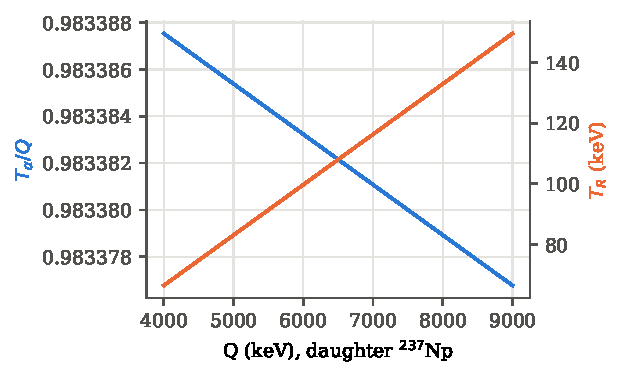
\includegraphics[width=0.62\linewidth]{fig/a_kin.pdf}
\caption{Fraction of the decay energy carried by the alpha (left axis) and the recoil energy (right axis) for a \nuc{237}{Np} daughter as a function of $Q$, using the exact kinematics of \cref{eq:exact}. The fraction is almost exactly $M_d/(M_d+m)$, decreasing very slightly with $Q$ (relativistic effect).}
\label{fig:akin}
\end{figure}

\begin{keyidea}[The recoil matters]
A \SI{100}{keV} nuclear recoil is an excellent mimic of a WIMP signal in a dark-matter detector. If the alpha is lost in a wall or a surface layer (e.g.\ \nuc{210}{Po} plated out on a detector surface) the recoiling \nuc{206}{Pb} can enter the active volume on its own. In liquid argon or xenon its scintillation is strongly quenched (Lindhard-type quenching factors of order 0.1--0.3), so a \SI{103}{keV} recoil looks like a few tens of keVee.
\end{keyidea}

\section{Where does the width of an alpha line come from?}
For a parent at rest, \cref{eq:exact} has no free parameter: the alpha is mono-energetic. The \emph{emission angle} in the centre-of-mass frame cannot broaden the line, because for a parent at rest the CM frame \emph{is} the lab frame and the energy does not depend on direction. The contributions to an observed width are:
\begin{enumerate}
\item \textbf{Natural width} $\Gamma = \hbar/\tau$. For any alpha emitter with a measurable half-life this is absurdly small ($\hbar = \SI{6.6e-16}{eV\,s}$).
\item \textbf{Fine structure.} Branches to daughter levels a few tens of keV apart (e.g.\ \nuc{241}{Am}: 5486, 5443 and \SI{5388}{keV}) are separate lines that merge at modest resolution.
\item \textbf{Motion of the parent} (\cref{sec:boost}): if the parent moves, the lab energy depends on the CM emission angle. This \emph{is} an emission-angle effect, and it is the only kinematic broadening.
\item \textbf{Energy loss before detection}: source self-absorption, dead layers, gas or windows. This produces a low-energy tail, not a symmetric width, and is usually the dominant effect in practice.
\item \textbf{Detector resolution}: Fano-limited charge statistics in silicon (\SIrange{10}{20}{keV} FWHM), or photostatistics and quenching fluctuations in a scintillator.
\item \textbf{Coincident summing}: the conversion electrons, X-rays or gammas from the daughter level, if absorbed in the same detector, add to the alpha energy (important for sources inside a calorimeter, such as alphas in a liquid-argon detector).
\end{enumerate}
The Alpha tab lets you set the detector resolution (item 5) and the parent kinetic energy (item 3).

\section{A moving parent: the flat box}
\label{sec:boost}
Suppose the parent moves with kinetic energy $T_p$, i.e.\ with Lorentz factor $\gamma = 1 + T_p/M$ and velocity $\beta = \sqrt{1-\gamma^{-2}}$. Let the alpha have energy $E^*$ and momentum $p^*$ in the parent rest frame (\cref{eq:exact}), emitted at angle $\theta^*$ to the boost direction. The Lorentz transformation gives
\begin{equation}
E_\text{lab} = \gamma\left(E^* + \beta p^* \cos\theta^*\right).
\label{eq:boost}
\end{equation}
Emission is isotropic in the parent frame (for unpolarised nuclei), so $\cos\theta^*$ is uniform on $[-1,1]$, and because \cref{eq:boost} is \emph{linear} in $\cos\theta^*$ the lab energy is \emph{uniformly} distributed between
\begin{equation}
E_\text{min,max} = \gamma\left(E^* \mp \beta p^*\right).
\label{eq:range}
\end{equation}
In the non-relativistic limit, writing $T^*$ for the CM kinetic energy and using $\beta p^* \approx \sqrt{2mT^*}\sqrt{2T_p/M}$,
\begin{equation}
T_\text{lab} \in \left[\left(\sqrt{T^*} - \sqrt{\tfrac{m}{M}T_p}\right)^2,\ \left(\sqrt{T^*} + \sqrt{\tfrac{m}{M}T_p}\right)^2\right],
\qquad \text{full width} \approx 4\sqrt{\frac{m}{M}\,T^* T_p}.
\label{eq:nrbox}
\end{equation}
\code{boostRange(Tstar, m, Mp, Tp)} returns the exact endpoints of \cref{eq:range}; the tab applies it to both the alpha and the recoil. \Cref{fig:band} shows the box for \nuc{210}{Po}.

\begin{figure}[htbp]
\centering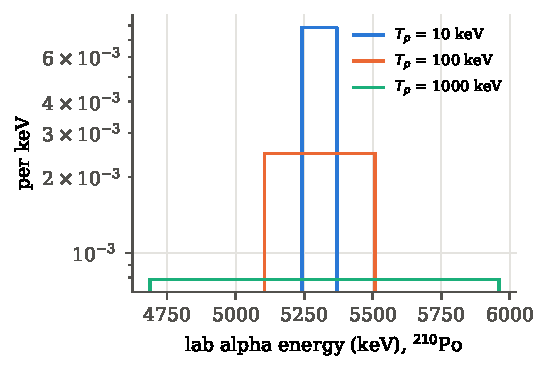
\includegraphics[width=0.62\linewidth]{fig/a_band.pdf}
\caption{Lab-frame alpha energy distribution from \nuc{210}{Po} for several parent kinetic energies $T_p$. A parent moving with \SI{100}{keV} (a typical recoil energy from a preceding alpha decay) spreads the line over \SIrange{5105}{5507}{keV}: \SI{400}{keV} wide, far more than detector resolution. The recoiling \nuc{206}{Pb} spans \SIrange{0}{402}{keV} in the same case.}
\label{fig:band}
\end{figure}

\begin{pitfall}[When does the box actually occur?]
A recoiling nucleus in a solid or liquid stops in picoseconds to nanoseconds. A boosted alpha line therefore requires the second decay to happen \emph{before} the first recoil stops, i.e.\ a daughter half-life well below a nanosecond (e.g.\ \nuc{212}{Po}, \SI{0.3}{\micro s}, is already far too slow in condensed matter, but is relevant in a dilute gas). The box is also the right description for decays in flight of beam-produced nuclei, and for $(\alpha,n)$ and other reaction kinematics (see the $(\alpha,n)$ note), where it is essential.
\end{pitfall}

\section{Lifetimes: Geiger--Nuttall in one paragraph}
The alpha is preformed inside the nucleus and tunnels through the Coulomb barrier. In the WKB approximation the decay rate is $\lambda = \nu P e^{-2G}$ with assault frequency $\nu\sim10^{21}\,\mathrm{s^{-1}}$, preformation factor $P$, and Gamow factor
\begin{equation}
G = \frac{1}{\hbar}\int_R^{b}\sqrt{2\mu\left(\frac{2Z_d e^2}{4\pi\epsilon_0 r} - Q\right)}\,\dd r
= \eta\left[\arccos\sqrt{x} - \sqrt{x(1-x)}\right] \approx \eta\left(\frac{\pi}{2} - 2\sqrt{x}\right),
\end{equation}
where $x = R/b$, $\eta = 2Z_d\,\alpha\,c/v = Z_d\,\alpha\sqrt{2\mu c^2/Q}$ is the Sommerfeld parameter, $\mu$ the reduced mass, $R$ the nuclear radius, and $b = 2Z_d e^2/(4\pi\epsilon_0 Q)$ the classical turning point. The leading term gives $\log_{10} t_{1/2} \approx a Z_d/\sqrt{Q} + c$ (Geiger--Nuttall): a factor of two in $Q$ changes the half-life by over twenty orders of magnitude. The same barrier-penetration physics explains why branches to excited daughter states (lower $Q - E_x$) and with angular momentum $\ell > 0$ (centrifugal barrier) are suppressed.

\section{What the Alpha tab outputs}
Given a parent, the tab lists every alpha branch with its intensity, daughter level and exact $T_\alpha$, $T_R$ (\cref{eq:exact}); draws the alpha and recoil spectra as lines (parent at rest) or boxes (\cref{eq:range}) convolved with a Gaussian detector resolution; and exports the formula and a CSV. The parent's $Q$ is looked up from the mass table when you type a nuclide.

\section{Exercises}
\begin{exercise}[A]
Derive \cref{eq:exact} and expand it to obtain \cref{eq:nr} plus the first relativistic correction. Evaluate the correction for \nuc{210}{Po} in eV.
\end{exercise}
\begin{exercise}[A]
Show that \cref{eq:boost} with isotropic $\cos\theta^*$ gives a flat distribution, and derive the non-relativistic box \cref{eq:nrbox}. What is the distribution of the lab \emph{angle}? (It is not isotropic.)
\end{exercise}
\begin{exercise}[A]
\nuc{212}{Bi} $\beta^-$-decays to \nuc{212}{Po}, which alpha-decays with $t_{1/2} = \SI{0.3}{\micro s}$ and $T_\alpha = \SI{8785}{keV}$. The \nuc{212}{Po} recoils from the beta decay with at most a few tens of eV. Estimate the width of the resulting box and compare with the range of the recoil in liquid argon. Is the box observable?
\end{exercise}
\begin{exercise}[P]
Using the mass excesses in \code{data/signals/nuclides.json}, compute $T_\alpha$ for every alpha branch of the \nuc{238}{U} chain and compare with the ENSDF values in the decay files. Plot the residuals; where are they largest, and why (hint: atomic vs.\ nuclear $Q$)?
\end{exercise}
\begin{exercise}[P]
Fit $\log_{10} t_{1/2}$ versus $Z_d/\sqrt{Q}$ for the even--even ground-state-to-ground-state alpha emitters in the database. Identify the outliers and explain them.
\end{exercise}
\begin{exercise}[R]
In a liquid-argon detector, \nuc{210}{Po} on the TPB-coated walls produces events with energies anywhere from a few keVee to the full alpha peak. Sketch the expected distribution, explaining the roles of the coating thickness, the recoil, and the different quenching of alphas and nuclear recoils.
\end{exercise}

\begin{thebibliography}{9}
\bibitem{ensdf} National Nuclear Data Center, ENSDF; IAEA LiveChart of Nuclides, \url{https://www-nds.iaea.org/livechart/}.
\bibitem{ame} M.~Wang \emph{et al.}, ``The AME 2020 atomic mass evaluation (II)'', Chin.\ Phys.\ C \textbf{45}, 030003 (2021).
\bibitem{krane} K.~S. Krane, \emph{Introductory Nuclear Physics} (Wiley, 1988), ch.~8.
\bibitem{hagedorn} R.~Hagedorn, \emph{Relativistic Kinematics} (Benjamin, 1963), ch.~7.
\end{thebibliography}
\end{document}
